\documentclass{article}

% Useful packages
\usepackage{amsmath}  % improve math presentation
\usepackage{amssymb}
\usepackage{amsthm}
\usepackage[english]{babel}
\usepackage{cancel}
\usepackage{caption}
\captionsetup{labelfont=bf, font=footnotesize}
\usepackage{circuitikz}
\usepackage{cite} % takes care of citations
\usepackage{enumitem}
\usepackage[final]{hyperref} % adds hyper links inside the generated pdf file
\hypersetup{
	colorlinks=true,       % false: boxed links; true: colored links
	linkcolor=black,        % color of internal links
	citecolor=blue,        % color of links to bibliography
	filecolor=magenta,     % color of file links
	urlcolor=blue         
}
\usepackage[utf8]{inputenc}
\usepackage[letterpaper,top=2cm,bottom=2cm,left=3cm,right=3cm,marginparwidth=1.75cm]{geometry}
\usepackage{graphicx} % takes care of graphic including machinery
\usepackage{placeins} % better float control
\usepackage{siunitx}
\sisetup{
    sticky-per,
    per-mode=power,
    exponent-product=\cdot,
    forbid-literal-units,
    inline-per-mode=power,
    display-per-mode=fraction,
    uncertainty-mode=separate,
    output-decimal-marker={,}
}
\usepackage{standalone}
\usepackage{subcaption}
\usepackage{tabularx} % extra features for tabular environment

%

\newcommand{\var}[2]{#1_\mathrm{#2}}

\theoremstyle{definition}
\newtheorem{example}{Example}

%

\title{Cookbook}
\author{Politek}

\begin{document}
\maketitle

\numberwithin{figure}{section}
\numberwithin{equation}{section}

\begin{abstract}
    This document provides an analysis of the behavior of each of the subcircuits that can be found in the kick, along with a quick summary for future reference.
\end{abstract}

\tableofcontents

\section{Gate to trigger}
Let's start from the very first block of the circuit.
The purpose of the \textit{gate to trigger} is to transform the signal from the sequencer into a sequence of short impulses.

\subsection{Analysis}
The input voltage \(v_i\) is the sequencer signal. It is a sequence of rectangular windows (gates).

\begin{figure}[ht]
    \centering
    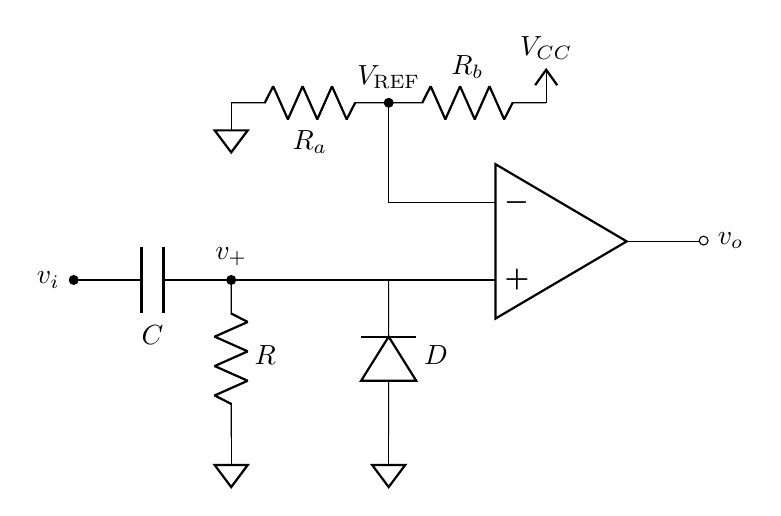
\begin{tikzpicture}
	% Paths, nodes and wires:
	\draw (7, 4) to[american resistor, l={$R$}, label distance=0.02cm] (7, 2);
	\draw (7, 4) to[capacitor, l={$C$}, label distance=0.02cm] (5, 4);
	\draw[draw] (7, 4) -- (10, 4);
	\draw (9, 2) to[empty diode, l_={$D$}, label distance=0.02cm] (9, 4);
	\draw node[sground] at (7, 2) {};
	\draw node[sground] at (9, 2) {};
	\draw node[circ] (N1) at (5, 4) {} node[anchor=east] at (N1.west){$v_i$};
	\draw node[op amp] at (11.19, 4.49) {};
	\draw (9, 6.25) to[american resistor, l={$R_b$}, label distance=0.02cm] (11, 6.25);
	\draw (9, 6.25) to[american resistor, l={$R_a$}, label distance=0.02cm] (7, 6.25);
	\draw node[vcc] (N2) at (11, 6.25) {} node[anchor=south] at (N2.north){$V_{CC}$};
	\draw node[sground] (N3) at (7, 6.25) {};
	\draw[draw] (12.38, 4.49) -| (13, 4.5);
	\draw node[ocirc] (Vo) at (13, 4.5) {} node[anchor=west] at (Vo.east){$v_o$};
	\draw[draw] (10, 4.98) -| (9, 6.25);
	\draw node[circ] (N4) at (7, 4) {} node[anchor=south] at (N4.north){$v_+$};
	\draw node[circ] (N5) at (9, 6.25) {} node[anchor=south] at (N5.north){$V_\text{REF}$};
\end{tikzpicture}
    \label{fig:gate-to-trigger}
    \caption{Gate to Trigger}
\end{figure}

The signal \(v_i\) goes first of all through an RC high-pass fitler, hence \(v_+\) takes on the characteristic exponential shape upon every rising or falling edge of \(v_i\).
The presence of \(D\) is needed because some op-amps undergo an effect called "phase inversion" if the voltage at either terminal becomes too negative; the diode blocks \(v_+\) at a fixed value during the falling edge of \(v_i\) (Figure \ref{fig:gate-to-trigger-conditioning}).

\begin{figure}[htp]
    \centering
    \includegraphics[width=0.7\textwidth]{../images/gatebase.png} 
    \caption{Signal conditioning}
    \label{fig:gate-to-trigger-conditioning}
\end{figure}

The op-amp is in a non inverting comparator configuration (without hysteresis):
\begin{align*}
    v_o &= \begin{cases}
        +\var{V}{CC}, & v_A > \var{V}{REF} \\
        -\var{V}{CC}, & v_A < \var{V}{REF} \\
    \end{cases}
    &
    \var{V}{REF} &= k \var{V}{CC}
    &
    k \triangleq \frac{R_a}{R_a + R_b}
\end{align*}

The cut-off frequency of the high-pass filter is \(f_0 = \frac{1}{2 \pi \tau}\), where \(\tau = RC\).
During the rising edge of \(v_i\), we get \(v_A > \var{V}{REF}\) for a small time \(\Delta t\).
During this interval the output of the comparator is \(\var{V}{CC}\).
%
Let's examine what happens during this transient:
\begin{align}
    v_A(t) > \var{V}{REF} & \implies
    V_I e^{-t/\tau} (t) > \var{V}{REF} = k \var{V}{CC} \geq 0,
    \quad t \ge 0 \nonumber \\
    & \implies 0 < t < \tau \log\frac{V_I}{k \var{V}{CC}} \triangleq \Delta t
    \label{eq:trigger-dt}
\end{align}

In order to have a working circuit we need to ensure that the slew rate of the op-amp be sufficiently high:
\[S_R \gg \frac{2 \var{V}{CC}}{\Delta t}\]

Futhermore, the presence of the op-amp guarantees a small output impedance \(\var{R}{out} \approx 0\).

\begin{example}
    Let's choose \(\Delta t = \frac{T}{10}\) where \(T\) is the gate duration.
    We need to make sure that \(\tau\) is sufficiently small compared to \(T\), e.g. \(\tau = \Delta t = \frac{T}{10}\):
    \begin{align*}
        &\cancel{\tau} \log\frac{V_I}{k \var{V}{CC}} = \cancel{\Delta t} \implies
        V_I = e \cdot k \var{V}{CC} \implies
        k = \frac{R_a}{R_a + R_b} = \frac{V_I}{e \var{V}{CC}} \\
        &\tau = RC \implies C = \tau/R = \frac{T}{10R}
    \end{align*}
\end{example}

\subsection{Summary}
\begin{itemize}
    \item \(v_i(t) = V_I, \quad 0 \le t \le T\)
    \item \(\var{V}{REF} = \frac{R_a}{R_a + R_b} \var{V}{CC}\)
    \item \(\Delta t = \tau \log\frac{V_I}{\var{V}{REF}}\)
    \item \(S_R \gg \frac{2\var{V}{CC}}{\Delta t}\)
\end{itemize}

\end{document}